\documentclass{standalone}
\usepackage{tikz}
\usetikzlibrary{shapes.geometric,patterns.meta}

\begin{document}
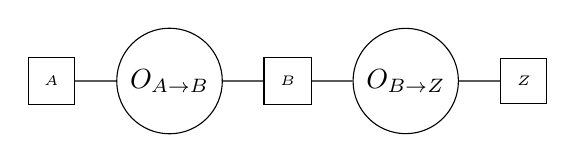
\begin{tikzpicture}[square/.style={regular polygon,regular polygon sides=4}]
    \node at (-1, 0) [circle, minimum size=0.8cm, draw] (cir) {$O_{A \rightarrow B}$};
    
    \node at (-2.5, 0) [square, draw] (s) {\tiny $A$};
    \node at (0.5, 0) [square, draw] (eb) {\tiny $B$};

    \node at (2, 0) [circle, minimum size=0.8cm, draw] (b) {$O_{B \rightarrow Z}$};
    
    \node at (3.5, 0) [square, draw] (ez) {\tiny $Z$};
    \draw (s.east) -- (cir.west); 
    \draw (cir.east) -- (eb.west);
    \draw (eb.east) -- (b.west);
    \draw (b.east) -- (ez.west); 
\end{tikzpicture}
\end{document}
